%! Author = Dean
%! Date = 12/28/2023

\chapter{Evolucija konvolucijskih neuronskih mreža}\label{ch:evolucija-konvolucijskih-neuronskih-mreza}
Konvolucijske neuronske mreže \emph{KNM} predstavlja ključnu inovaciju u području analize slika i obrade vizualnih podataka.
U posljednjem razdoblju, KNM arhitektura doživjela je značajan tehnološki napredak.
Ovaj napredak omogućio je postizanje rezultata koji su prije bili nezamislivi, često se približavajući ili čak nadmašujući ljudske sposobnosti u određenim zadacima vizualne analize.
Današnje vrijeme karakterizira raznolikost KNM-ova, s različitim arhitekturama koje su prilagođene specifičnim zadatcima.
Svaka arhitektura ima svoje prednosti i mane, a \enquote{Teorem besplatnog ručka} ukazuje na to da nema univerzalno najbolje arhitekture.
Zato ćemo sada malo proći kroz evoluciju konvolucijskih neuronskih mreža od samih početaka pa do danas.

\section{Neocognitron}\label{sec:neocognitron}
Možemo reći da je Neocognitron preteča konvolucijskih neuronskih mreža.
Ova arhitektura je prva uvela pojmove kao što su ekstrakcija značajki (\emph{feature extraction}), konvolucija (\emph{convolution}), i slojevi uzorkovanja (\emph{pooling layers}).
\FloatBarrier
\begin{figure}[h]
    \centering
    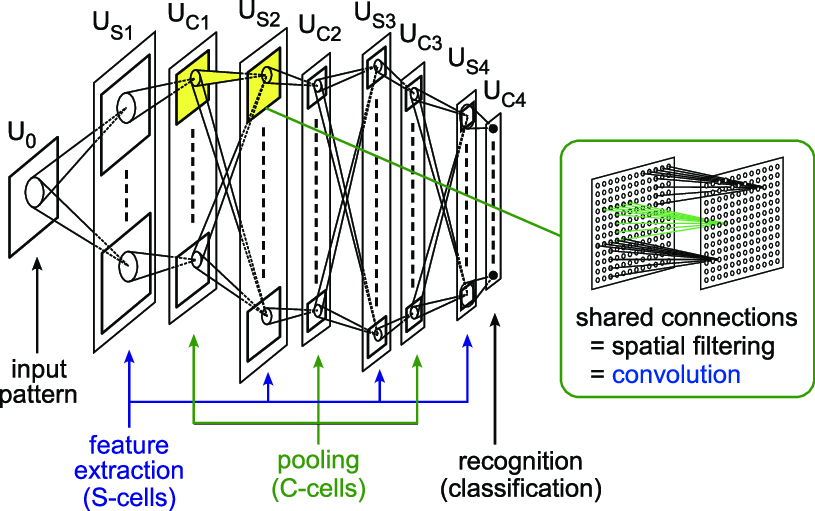
\includegraphics[width=0.6\textwidth]{images/Neocognitron}
    \caption{Arhitektura Neocognitron}
    \label{fig:slika7}
\end{figure}
\FloatBarrier
Arhitektura Neocognitrona sastoji se od alternirajućih S i C slojeva, pri čemu svaki od njih sadrži S i C stanice.
S stanice, ili jednostavne stanice, služe za detekciju lokalnih značajki, dok C stanice, ili kompleksne stanice, služe za dodavanje tolerancije prema samoj poziciji objekta.
Na taj način dobivamo model koji je invarijantan na translacijske promjene, odnosno trebao bi prepoznati oblik bez obzira na to gdje se nalazi na slici.

\section{LeNet-5}\label{sec:lenet-5}
LeNet-5 je dizajnirana od strane francuskog informatičara Yanna LeCuna između 1989. i 1998. godine i postigla je uspjeh u prepoznavanju rukom pisanih brojeva.

Arhitektura se sastojala od tri konvolucijska sloja i dva sloja za uzrokovanje koji su bili međusobno alternirajući. Na kraju su se nalazila dva potpuno povezana sloja.

U konvolucijskim slojevima koristio se 5x5 filter s korakom veličine 1, odnosno s pomakom veličine 1. S druge strane, slojevi za uzrokovanje bili su 2x2 s pomakom veličine 2.
\begin{figure}[h]
    \centering
    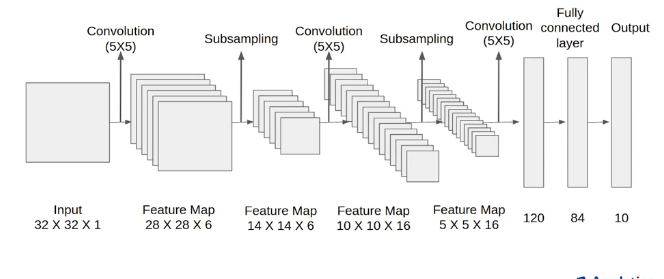
\includegraphics[width=0.6\textwidth]{images/LeNet}
    \caption{Arhitektura LeNet-5.}
    \label{fig:slika8}
\end{figure}
Dimenzija ulazne slike je 32x32x1 jer se ova arhitektura uglavnom koristila za prepoznavanje rukom pisanih brojeva. Dimenzije označavaju širinu, visinu i dubinu slike. Za crno-bijele slike dubina je 1, što znači da postoji samo jedan kanal. Za RGB slike, dubina bi bila 3 (jedan kanal za crvenu, zelenu i plavu komponentu svake boje).

Prvi konvolucijski sloj ima 6 filtera veličine 5x5 s pomakom od 1.
Rezultat tog sloja je značajka veličine 28x28x6.
Izlazni sloj se može izračunati pomoću formule: \[ \textit{dimenzija} = \frac{\textit{ulazna dimenzija} - \textit{veličina filtera}}{\textit{korak}} + 1 \].

Nakon toga slijedi sloj za uzrokovanje veličine 2x2.
Ovdje se koristi average pooling koji za vrijednost uzima prosjek od odabrane 4 vrijednosti.

Dalje slijede još dva konvolucijska sloja, jedan sloj za uzrokovanje i dva potpuno povezana sloja, od kojih je jedan izlazni sloj.
Izlazni sloj sastoji se od 10 neurona i koristi Softmax kao aktivacijsku funkciju.
Softmax je prikladan jer za svaku klasu daje vjerojatnost da ulaz pripada toj klasi, a predikcija se izvodi tako da se odabere klasa s najvećom vjerojatnošću.

